For a classification task it is required that a model can output a prediction.
This prediction can for example simply by a discrete class label,
but also a probability distribution. 
In \nenwin it is straightforward to obtain a one-hot-encoding of discrete class label as output, by using MarbleEaterNodes.
In this case, the output will simply be a vector of integers, 
where each value represents the number of Marbles eaten by each MarbleEaterNode.
The MarbleEaterNodes may be ordered in any arbitrary fix order, as long as, at each point in time $t = t_j$, 
the output can be interpreted as an array with one value for each MarbleEaterNode.

This can be expressed more formally as defining a \textit{cumulative output vector}:
\begin{definition}[cumulative output vector] \label{def:cumul_output_vect}
Given a \nenwin model $M$, then for each point in time $t$, define the \textbf{cumulative output vector} $\vec{M}(t)$ as:
\begin{equation}
    \vec{M}(t)_i \equiv \text{number of Marbles eaten by the $i^{th}$ MarbleEmitterNode at time $t$}
\end{equation}
\end{definition}
Note that $\vec{M}(t)$ is always a vector of nonnegative integers, and at $t = 0$ we have $\vec{M}(0) = \vec{0}$.


\subsection{Loss definition}
The output of the model changes over time, and hence it is practical to define the 'real' output $\hat{\vec{y}}$ as the time-varying output read at a certain point in time. For convenience, call this time $t_{end}$. Then \begin{equation}
    \hat{y} \equiv \vec{M}(t_{end})
\end{equation} Given an expected output $\vec{y}$, the most straightforward way to define the \textit{loss} of the 'real' output $\hat{\vec{y}}$ is to take a measure of difference between $\vec{y}$ and $\hat{\vec{y}}$, such as the Mean Squared Error or the Cross Entropy Loss. However, this approach is not optimizable in all situations, as explained below.

\subsubsection{Classification loss}
Consider an application where a \nenwin model is used to classify an input as one out of $k$ classes. Let each class-prediction be represented by a single MarbleEaterNode. Now since only one class is needed, the output $\hat{\vec{y}}$ can be read when the first Marble is eaten, or when the time $t = t_{max}$. More formally, let 
\begin{equation}
    t_{end} \leftarrow \min \left(\{t \; | \; 1 \leq \norm{\vec{M}(t)}\}\cup \{t_{max}\}\right).
\end{equation}
Now there are three possible cases for the output $\hat{\vec{y}}$ 
(for now, assume only one Marble will be eaten at $t = t_{end}$):
\begin{enumerate}
    \item $\hat{\vec{y}} = \vec{y}$, and the loss can be set to 0.
    \item $t_{end} = t_{max}$ and $\hat{\vec{y}} = \vec{0}$, that is, no Marble has been eaten.
    \item $\hat{\vec{y}} \neq \vec{y}$ (and $\hat{\vec{y}} \neq \vec{0}$).
\end{enumerate}

In case 2, it is expected that a Marble arrived at a specific MarbleEmitterNode $n$. However, there may be multiple Marbles present in the model, hence it is not clear \textit{which} Marble should be eaten by $n$ to achieve the desired output. 
The chosen method to resolve this is choosing the Marble $m$ for which the loss would be smallest.
Intuitively, this method 'blames' the Marble that seems most promising to be eaten by $n$ for the loss.
More formally, define:
\begin{equation}
    L(\hat{\vec{y}}, \vec{y}) = \smashoperator{\min_{m \in Marbles}} \; f(m, n, t_{end}) \label{eq:classification_loss_net}
\end{equation}
where
\begin{equation}
    f(m, n, t) = \big\Vert{n.pos(t) - (m.pos(t) + \mu \cdot m.vel(t))}\big\Vert_2^2, \qquad \mu \in \mathbb{R}_{\geq 0}. \label{eq:classification_loss_one_marble}
\end{equation}
Here $\mu$ is a nonnegative real number that functions as a hyperparameter. 

The rationale behind including the '$+ \mu \cdot m.vel$' term is as follows: 
if only the position of the Marble is optimized, 
then it will be closer to $n$ at $t = t_{end}$, 
but this does not necessary imply it is also closer to being eaten by $n$. 
'Almost being eaten' also requires $m$ to be moving towards $n$!
'$+ \mu \cdot m.vel$' can be seen as a very naive prediction of the future position of $m$. 
The intent of this addition is to make it more likely that 'minimizing the loss function' correlates with 'making $m$ being eaten by $n$'.

$\mu$ could be fixed as a hyperparameter, but this may cause undesired effects when the  magnitude of $m.vel$ changes significantly. For example, if $\norm{m.vel}$ and $\mu$ are both large, then $m.pos + \mu \cdot m.vel$ might be further from $n.pos$ than $m.pos$, even if the direction of $m.vel$ is from $m.pos$ towards $n.pos$ (i.e. the naive prediction \textit{overshoots}). It may be wise to make $\mu$ a function of the magnitude of $m.vel$, e.g. to demand that $\mu \propto \frac{1}{\norm{m.vel}}$.

For case 3, also \eqref{eq:classification_loss_net} can be used for the missing Marble at the expected output MarbleEaterNode encoded in $\vec{y}$. However, there is also another Marble, $m'$, which was eaten by some node $n' \neq n$ (otherwise case 3 would equal case 2 or case 1), where $n'$ is the MarbleEaterNode at the unique index $i$ where $\hat{y}_i = 1$. Since $m'$ is eaten at $t = t_{end}$, $f(m', n', t_{end})$ (using \eqref{eq:classification_loss_one_marble}) is well defined, and the following loss function would penalize $m'$ moving towards $n'$:

\begin{equation}
    L(\hat{\vec{y}}, \vec{y}) = - \frac{1}{f(m', n', t_{end})} + \smashoperator{\min_{m \in Marbles}} \; f(m, n, t_{end})
\end{equation}

The reciprocal $- \frac{1}{f(m', n', t_{end})}$ is used instead of $f(m', n', t_{end})$, 
as the latter will be small in magnitude (considering the Marble was eaten), 
but becomes larger the further $m'$ is away from $n'$. 
But the further $m'$ is away from $n'$, the less $m'$ should be corrected.

It is possible to add scalar weights to each of the two terms 
$- \frac{1}{f(m', n', t_{end})}$ and $\min_{m \in marbles} f(m, n, t_{end})$, 
but this approach has not been explored further.

In summary, the loss $L(\hat{\vec{y}}, \vec{y})$ is defined as:
\begin{equation}
    L(\hat{\vec{y}}, \vec{y}) = \begin{cases}
        0 & \text{if } \hat{\vec{y}} = \vec{y} \\
        - \frac{1}{f(m', n', t_{end})} + \min_{m \in Marbles} f(m, n, t_{end}) & \text{if } \vec{y} \neq \hat{\vec{y}} \neq \vec{0}  \\
        \min_{m \in Marbles} f(m, n, t_{end}) & \text{if } \hat{\vec{y}} = \vec{0}\\
    \end{cases}
    \label{eq:classification_loss_full}
\end{equation}
Where $n$ is the node at the unique index $i$ where $y_i = 1$, $Marbles$ is the set of all Marbles in the model, and $m'$ is \textit{the} Marble eaten by some node $n' \neq n$ in the case $\vec{y} \neq \hat{\vec{y}} \neq 0$.

\subsubsection{Multiple outputs}
Eq. \eqref{eq:classification_loss_full} assumes that at most one Marble will be eaten. 
It is possible that multiple Marbles will be eaten at the same time. 
Especially in simulation this is not unlikely, where discrete finite-sized time steps are taken.

Let $k$ be the number of Marbles eaten at $t = t_{end}$, and let these Marbles be $m_1, m_2, \dots, m_k$. 
Let the corresponding MarbleEaterNodes that ate them be $n_1, n_2, \dots, n_k$. 
Note that these MarbleEaterNodes may not all be distinct, while the Marbles are all unique. 
Let $n$ be the MarbleEaterNode of the correct (expected) output. 
Then we can extend \eqref{eq:classification_loss_full} to:
\begin{equation}
	L_{total}(\hat{\vec{y}}, \vec{y}) = \mathbbm{1}(n\notin \{n_1, n_2, \dots, n_k\}) \cdot \smashoperator{\min_{m \in Marbles}} f(m, n, t_{end}) 
									  - \sum_{i=1}^{k}   \frac{1}{f(m_i, n_i, t_{end})}
\end{equation}
Where $\mathbbm{1}(p)$ equals 1 if the proposition $p$ is true, and 0 if $p$ is false.
In the very specific case that \textit{all} Marbles have been eaten by the wrong Nodes,
the term $\min_{m \in Marbles} f(m, n, t_{end})$ will not be defined. 
It was chosen to simply leave this term out in this case. 
If the penalty for the wrongly eaten Marbles causes sufficient change in the update rule, 
then (in the next iteration, or a few iterations later) 
there will be uneaten Marbles available to 'blame' for not being eaten by the correct MarbleEaterNode.

In other words:
\begin{itemize}
	\item For each wrongly outputted Marble, the wrong-output penalty is added to the loss.
	\item In case the correct output was not included, also the missing-output penalty is added once.
\end{itemize}

Note that this method does not penalize multiple Marbles arriving at the correct output Node, 
which may in some contexts also be undesirable.

\subsubsection{Non-convexity}
Eq. \eqref{eq:classification_loss_full} is not convex. This is not surprising given its relatively complex piece-wise definition. 
%To simplify the notation, define the following extension of Definition \ref{def:cumul_output_vect}:
%
%\begin{definition}[Parametrized cumulative output vector]
%    Let $\vec{M_{\theta}}(t)$ denote the \emph{cumulative output vector} $\vec{M}(t)$ of a \nenwin architecture whose initial particles are described by $\theta$.
%\end{definition}

The following lemma proofs that even optimizing the initial values (which are the initial position, velocity, acceleration and the mass) of particles, keeping the set of particles themselves constant, does not have a convex objective.
\begin{lemma}[Non-convexity of \eqref{eq:classification_loss_full}]
Assuming a constant vector $\vec{y}$, \eqref{eq:classification_loss_full} is not convex, for all \nenwin architectures, in the \emph{initial values} of the particles.
\label{lemma:nonconvexity_loss}
\end{lemma}
\begin{proof}
For simplicity, we proceed with a specific counter-example. 
Consider an architecture with a single Marble $m$, two MarbleEmitterNodes $E_1$ and $E_2$, and a MarbleEaterNode $n$.
Let $\vec{y} = [1]$. 
Let both emitters have such a threshold and such a prototype that if they eat $m$, 
they will emit some new Marble $m'$ that will move towards $n$ and be eaten in $t' < \frac{1}{2}t_{end}$ time. 
Let $m.node\_stiffness = 1$. 
Now position the four initial particles on the vertices of a sufficient large square that their radii do not overlap, 
and $E_1$ and $E_2$ oppose each other. 
Let $A$ be the vertex assigned to $m$. 
The parameter of interest is now the initial velocity of $m$, in particular the \emph{angle} of $m.vel(t_0)$. 
Let the magnitude of $m.vel$ be such that, under constant $\vec{0}$ acceleration and no obstacles, 
$m$ would travel several times the length of an edge of the square. 
Now define the following angles $a_1 < a_2 < \dots < a_7$ of the direction of $m.vel$ (see Fig. \ref{fig:nonconvexity_loss}):
\begin{itemize}
    \item $a_2$: $m.vel$ is directed towards $E_1$, then $E_1$ would emit a Marble which arrives at $n$ before $t = t_{end}$. Hence the loss would be 0.
    \item $a_3$: $m.vel$ is directed towards the center of the edge of the square between $E_1$ and $n$. At $t = t_{end}$, $m$ would still exist and be far from $n$, and hence the loss would be much greater than 0.
    \item $a_4$: $m.vel$ is directed towards $n$ and $m$ will be eaten by $n$ before $t = t_{end}$, the loss will be 0.
    \item $a_5$: $m.vel$ is directed towards the center of the edge of the square between $E_2$ and $n$. The loss of this case is the same as in case 2 (i.e. nonzero).
    \item $a_6$: $m.vel$ is directed towards $E_2$. The loss of this case is 0, by symmetry with case 1.
    \item $a_1$ or $a_7$: $m.vel$ is not directed to the inside of the square, nor parallel or close to parallel to one of the edges, nor to one of the regions within the radii of $E_1$ or $E_2$. The loss will be nonzero as $n$ will not eat any Marble.
\end{itemize}
$\hat{\vec{y}}$ is a function of the initial values of the particles and the angle of $m.vel$ is part of these initial values. The loss in the case of $a_3$ is larger than in the case of $a_2$ or $a_4$ (see also Fig. \ref{fig:nonconvexity_loss_plot}). Clearly this violates the convexity property, and hence \eqref{eq:classification_loss_full} is not convex in the angle of $m.vel$, and hence not in all initial values of the particles.
\end{proof}

\begin{figure}[h]
    \centering
    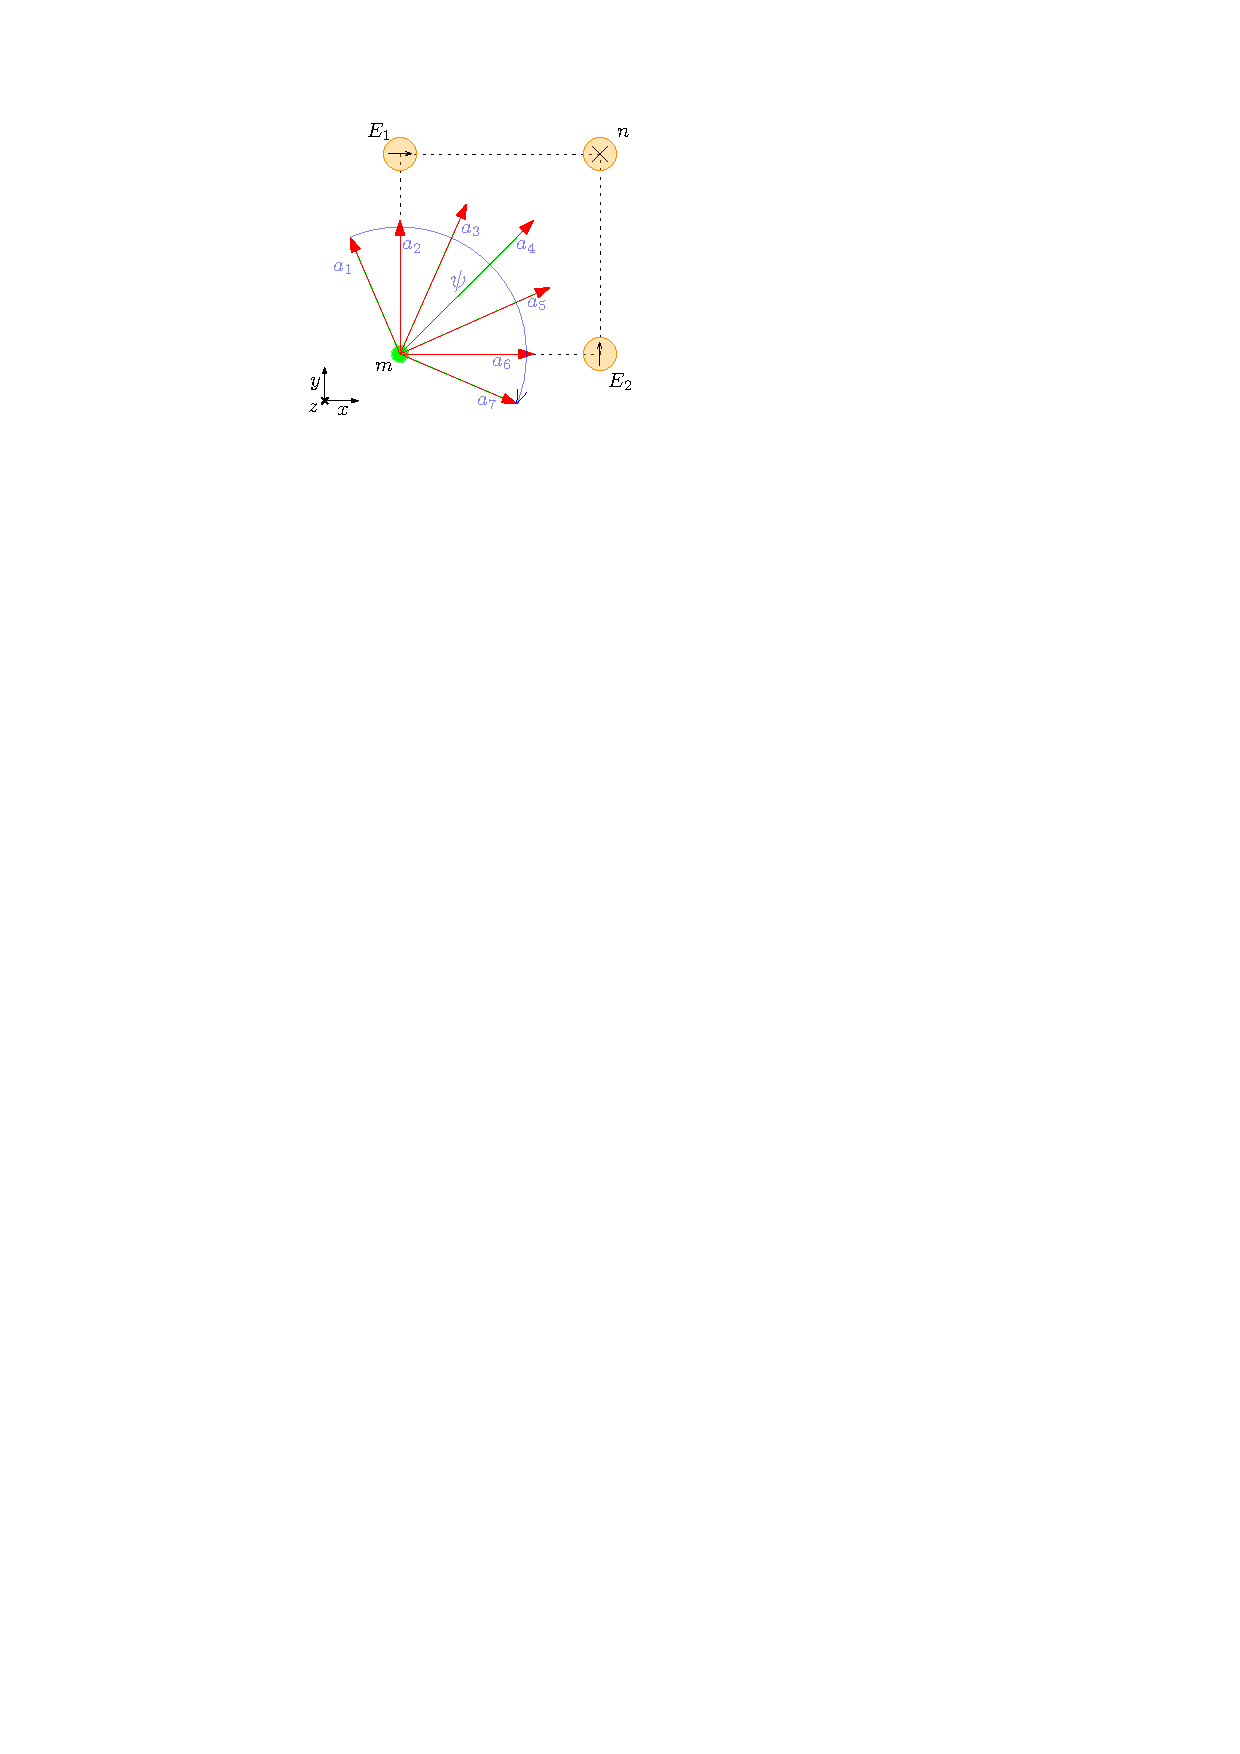
\includegraphics{figures/nonconvexity_of_loss.pdf}
    \caption{Sketch depicting the architecture used in the proof of Lemma \ref{lemma:nonconvexity_loss}. The red arrow depict the various angles $\psi$ of the direction of $m.vel$.}
    \label{fig:nonconvexity_loss}
\end{figure}

\begin{figure}
    \centering
    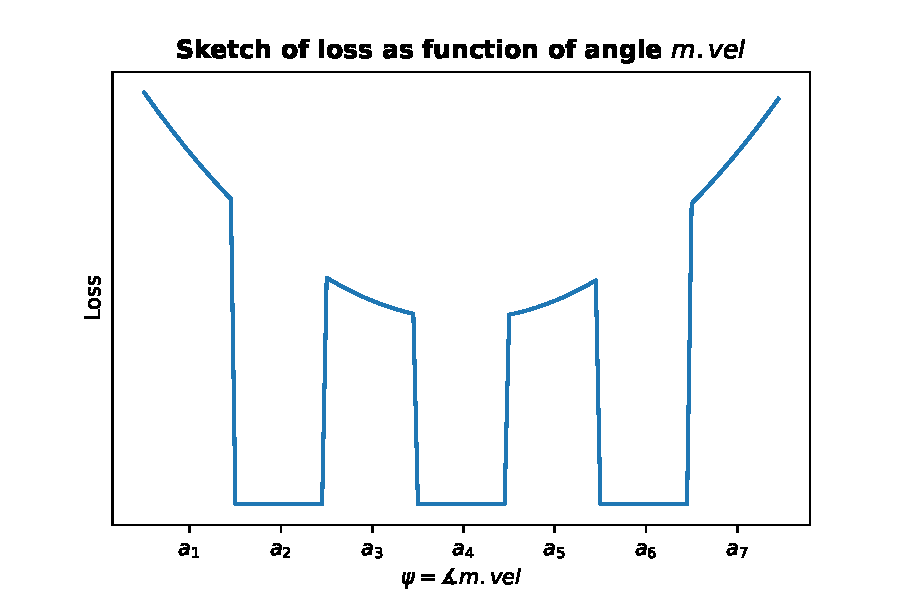
\includegraphics{plot_nonconvex_loss.pdf}
    \caption{Sketch depicting loss function $L(\hat{\vec{y}}, \vec{y})$ as a function of the angle $\psi$ of $m.vel$, in the architecture used in the proof of Lemma \ref{lemma:nonconvexity_loss}.}
    \label{fig:nonconvexity_loss_plot}
\end{figure}

\clearpage

\subsubsection{Loss gradient}

Let $p$ and $s$ be particles, then define the $stiffness$ function as:
\begin{equation}
    stiffness(p, s) = 
    \begin{cases}
        p.\texttt{marble\_stiffness} &\text{if $s$ is a Marble} \\
        p.\texttt{node\_stiffness} &\text{if $s$ is a Node} \\
    \end{cases}
\end{equation}


Using Eq. \eqref{eq:def_pos}, \eqref{eq:def_vel}, \eqref{eq:def_f_net} and \eqref{eq:def_acc} to describe the state of some particle $p$ at a point in time $t=t_1$, we can rewrite the state as follows (assuming that the amount of particles in the architecture is finite):
\begin{align}
    p.pos(t = t_1)  &= p.pos(t = t_1 - 0) + 0 
                    = \lim_{\varepsilon \downarrow 0}\Big(p.pos(t = t_1 - \varepsilon) + p.vel(t = t_1 - \varepsilon) \cdot \varepsilon \Big) \label{eq:pos_eps}\\
    p.vel(t = t_1)  &= p.vel(t = t_1 - 0) + 0 
                    = \lim_{\varepsilon \downarrow 0}\Big(p.vel(t = t_1 - \varepsilon) + p.acc(t = t_1 - \varepsilon) \cdot \varepsilon \Big) \label{eq:vel_eps} \\
    p.acc(t = t_1)  &= \smashoperator{\sum_{\substack{\text{particles $s$}\\\text{ acting on $p$}}}}stiffness(p, s)\cdot\frac{p.mass \cdot s.mass}{p.pos(t=t_1 + 0)-s.pos(t=t_1 + 0)} \nonumber \\
    &= \lim_{\varepsilon \downarrow 0}\Big(\smashoperator{\sum_{\substack{\text{particles $s$}\\\text{ acting on $p$}}}}stiffness(p, s)\cdot\frac{p.mass \cdot s.mass}{p.pos(t=t_1 -\varepsilon)-s.pos(t=t_1 -\varepsilon)}\Big) \label{eq:acc_eps}
\end{align}

Limits cannot be numerically represented on a digital computer. However, we can use a small finite-valued $\varepsilon > 0$, $\varepsilon \in \mathbb{R}$, and then it \textit{approximately} holds that:
\begin{align}
    p.pos(t = t_1)  &= p.pos(t = t_1 - 0) + 0 
                    \approx p.pos(t = t_1 - \varepsilon) + p.vel(t = t_1 - \varepsilon) \cdot \varepsilon \label{eq:pos_eps_approx}\\
    p.vel(t = t_1)  &= p.vel(t = t_1 - 0) + 0 
                    \approx p.vel(t = t_1 - \varepsilon) + p.acc(t = t_1 - \varepsilon) \cdot \varepsilon \label{eq:vel_eps_approx} \\
    p.acc(t = t_1)  &\approx \smashoperator{\sum_{\substack{\text{particles $s$}\\\text{ acting on $p$}}}}stiffness(p, s)\cdot\frac{p.mass \cdot s.mass}{p.pos(t=t_1 -\varepsilon)-s.pos(t=t_1 -\varepsilon)} \label{eq:acc_eps_approx}
\end{align}

Furthermore, note that for some $t_1 > t_0$, where $t_0$ is the starting time (at which each initially existing particle has its original position and velocity):
\begin{align}
    p.pos_0 &= p.pos(t=0) = p.pos(t = t_1 - t_1) \approx p.pos(t = t_1 - \varepsilon \varrho t_1) \label{eq:end_of_recursion}
\end{align}
for some positive constant $0 < \varrho < 1$ defined such that $\varrho t_1 \in \mathbb{Z}$.

We can use the above approximations to rewrite the position of a particle $p$ as a recursive function though time depending on earlier states:

\begin{align}
    p.pos(t = t_1)  &= p.pos(t = t_1 - 0) + 0 
                    \approx p.pos(t_1 - \varepsilon) + \varepsilon \cdot p.vel(t_1 - \varepsilon) \nonumber \\
                    &\approx p.pos(t_1 - \varepsilon) + \varepsilon \Big(  p.vel(t_1 - 2\varepsilon) + \varepsilon \cdot p.acc(t_1 - 2\varepsilon) \Big)\nonumber \\
                    &\approx p.pos(t_1 - \varepsilon) + \varepsilon \Big(  p.vel(t_1 - 2\varepsilon) \nonumber \\ &+ \varepsilon \cdot \smashoperator{\sum_{\substack{\text{particles $s$}\\\text{ acting on $p$}}}}stiffness(p, s)\cdot\frac{p.mass \cdot s.mass}{p.pos(t=t_1 -3\varepsilon)-s.pos(t=t_1 -3\varepsilon)} \Big) \label{eq:pos_recursive}
\end{align}
The terms $p.pos(t=t_1 - 2\varepsilon)$ and $p.vel(t = t_1 - 2\varepsilon)$ can again be expanded using \eqref{eq:pos_eps_approx} and \eqref{eq:vel_eps_approx}. Assume that no MarbleEmitterNodes are present and no inputs are given. Consider the scenario where one continues this process, and applies \eqref{eq:end_of_recursion} where this approximation is reasonable. If no circular recursion occurs (i.e. the sequence of substitutions does not produce a term that was previously substituted), then eventually an expression will be obtained in only the variables $k.mass$ and $k.pos_0$ for all particles $k$ in the architecture. These variables are adjustable parameters, and the applied operations are division, multiplication and subtraction. Hence is the desired output time and location are known, then the Backpropagation algorithm can be applied, in combination with, for example, Gradient Decent, to optimize the architecture.

Now let $m$ be an input that is given to the architecture at some time $t_{input} > t_0$. Let $m.pos_0 = m.pos(t_{input})$. Using Eq. \eqref{eq:pos_eps_approx}, \eqref{eq:vel_eps_approx} and \eqref{eq:acc_eps_approx}, which are all differentiable, we can recursively compute $\frac{\partial L}{\partial m.pos_0}$. Now recall that a \nenwin instance is defined with a function that maps external data to input Marbles (the \texttt{placement\_funct} argument in the pseudocode Algorithm \ref{alg:Nenwin_V1}). If this function has learnable parameters, then $\frac{\partial L}{\partial m.pos_0}$ depends on those, and hence Backpropagation can optimize the function's parameters via $\frac{\partial L}{\partial m.pos_0}$.

\subsection{Backpropagation of mass-gradient through MarbleEmitterNodes}
Now consider a Marble $m$ that is produced by a MarbleEmitterNode $n$. Let $n.spawnpos$ be the relative position of $m$ with respect to $n$ when $m$ was emitted, and $m.pos_0$ be the absolute position where $m$ was spawned. Now $m.spawnpos$ and $m.mass$ are parameters of $n$, and $n$ is initially present in the architecture. 
A difficulty arises, since $m.pos_0$ depends on the time $t = \hat{t}_0$ at which $m$ was created, which depends on on the \texttt{stored\_mass} of $n$. 
$n.stored\_mass$ can be seen a non-smooth function of time and the set of consumed Marbles
(which in turn depend on their initial position, attraction by other particles, their mass, etc.):
\begin{equation}
    n.stored\_mass(t) = \qquad \smashoperator{\sum_{k \in n.eaten\_marbles}} k.mass \qquad - \qquad \smashoperator{\sum_{h \in emitted\_marbles(n)}} h.mass \geq 0
\end{equation}
Where $emitted\_marbles(n)$ denotes the set of Marbles previously emitted by $n$. 
This set only exist conceptually: no variable or attribute has been defined to track it.


One way to resolve this issue is to see the \texttt{stored\_mass} 
together with the mass of the stored Marbles and the emitted mass as one continuum. 
In this case, $m.pos_0$ only depends on the last $x$ consumed Marbles by $n$ at $t = \hat{t}_0$ that together have sufficient mass, i.e.
\begin{equation}
    x = \min_{\hat{x} \in \mathbb{Z}} (\hat{x} : \left(\sum_{i = \hat{x}}^{\norm{n.eaten\_marbles(\hat{t}_0)}} n.eaten\_marbles(\hat{t}_0)[i].mass\right) \geq m.mass )
\end{equation}
where we use the fact that $n.eaten\_marbles$ is a stack with references to the Marbles consumed by $n$. For convenience, call this set of $x$ Marbles $X$.

Now between being consumed and being emitted, the quantity of mass that is $m.mass$ is 'frozen': it does not take part in any multiplication (except for the comparison whether $m$ can already be emitted). Hence, under the assumption that $m.mass$ directly depends on the mass of the last $x$ consumed Marbles (before $m$ was emitted), and that inclusion in this set $X$ directly depends on the \textit{last} position of each Marble in $X$. It will be assumed that these direct dependencies can be modelled with a derivative of 1, i.e. for all $m_i \in X$ that are consumed by $n$ at time $t_i$:
\begin{align}
    \frac{\partial m.pos_0}{\partial m_i.mass} = 1 \label{eq:deriv_emitted_to_mass}\\
    \frac{\partial m.pos_0}{\partial m_i.pos(t_i)} = 1 \label{eq:deriv_emitted_to_pos}
\end{align}
Eq. \eqref{eq:deriv_emitted_to_mass} and \eqref{eq:deriv_emitted_to_pos} are the 'missing link' that allows Backpropagation though MarbleEmitterNodes. Note that strong assumptions have been made, that need to be justified by experimental results\footnote{This will remain a topic for further research, as a better approach might be desirable.}. 
A disadvantage of this approach is that $n.radius$ is considered to be fixed, and cannot be optimized.

% The derivatives of $m.pos_0$ with respect to the other parameters of the MarbleEmitterNode itself can directly be computed, using the definition of $m.pos_0$: 
% \begin{align}
%     m.pos_0 = n.spawnpos + n.pos(t = \hat{t}_0) \\
%     \frac{\partial m.pos_0}{n.spawnpos} = 1 \\
%     \frac{\partial m.pos_0}{n.pos(\hat{t}_0)} = 1
% \end{align}

\subsection{Backpropagation of pos-, vel- and acc-gradient through MarbleEmitterNodes}
The above description allows to find the gradient of the mass of an emitted Marble $m$ with respect to the Marbles consumed by the MarbleEmitterNode $n$, and $n$ itself. But also the gradient of the loss with respect to the initial position of the Marble can be used to optimize $n$. Note that $m$ is created when certain variables (the time passed since last emit and $\norm{n.stored\_mass}$) exceed a certain threshold ($n.delay$ and $\norm{m.mass}$). 
\begin{align}
    m.pos_0 &= n.pos(t) + n.spawnpos \\
    \frac{\partial m.pos_0}{\partial n.pos(t)} &= \vec{1} \\
    \frac{\partial m.pos_0}{\partial n.spawnpos} &= \vec{1}
\end{align}

\subsection{Non-propagatable gradients}

The position and the mass are special cases where the gradient of a loss with respect to a variable of the emitted Marble can be propagated back to the MarbleEmitterNode and the particles that influenced the MarbleEmitterNode. For other variables of the Marble, such as the initial velocity and acceleration, this does not seem to be the case. The acceleration is a function of the particles that are present in the neighbourhood of the place where the Marble is created, hence it is intuitive that this is not differentiable to the MarbleEmitterNode. For the velocity (and any other ordinary variable that extensions of Marbles may have) this might less intuitive.

It can be shown by using a general case. Consider an object with variable $v$ is created at a certain point in time $\hat{t} > 0$ where some time-varying variable $x(t)$ meets a certain threshold $\theta$. Then initial value of $v$ at $\hat{t}$, $v_0$, can be written as a function of $\theta$ and $x$. Let $\hat{v}$ be the predefined value that becomes \textit{assigned} to $v$ at $t = \hat{t}$. Note that \textit{the value of} $v_0$ is independent of the value of $x(t)$ and vice-versa ($v_0$ is only created when $x(t) \geq \theta$, hence we always have $ReLU(\text{sgn}(\norm{x(\hat{t}) - \theta})) = 1$ when $v_0$ is created).

We have 
\begin{align}
    v_0 &= v_0(x(t), \theta) = \hat{v} \cdot ReLU(\sgn(\norm{x(\hat{t}) - \theta})) \\
    \frac{\partial v_0}{\partial x} &= \hat{v} \cdot \frac{\partial ReLU}{\partial \text{sgn}} \cdot \frac{\partial \text{sgn}}{\partial x} \\
    \frac{\partial v_0}{\partial \theta} &= \hat{v} \cdot \frac{\partial ReLU}{\partial \text{sgn}} \cdot \frac{\partial \text{sgn}}{\partial \theta}
\end{align}
\hl{Add arguments to ReLU and sgn!}

%\subsubsection{Backpropagation with inputs}
% \hl{
% Hence Eq. \eqref{eq:end_of_recursion} still applies, only with a different value of $\varrho$ than for particles that are initially already present in the architecture. However, the moment in time at which $m$ is created also depends on the Marbles $n$ has consumed earlier. For a correct optimization, Backpropagation needs to propagate though these Marbles as well.

% Let $\frac{\partial L}{\partial m.pos_0}$ be the gradient of the computed loss function with respect to the position where $m$ was 'spawned' at the time $t = \hat{t}_0$ when $m$ was created. Any Marble $k$ that had not been consumed by $n$ at time $t = \hat{t}_0$ had no direct influence on the creation 

% Also for input Marbles 
% }

\subsection{Backpropagation discussion}
The training theory described above can only be applied if an output has been received. If no output is provided by the architecture, then it is ambiguous which Marble was required to be consumed by a specific MarbleEaterNode at a specific point in time. To resolve this, it is possible to assign a particular Marble a priori to be the output, or design the architecture in such a way that an output will always be given after sufficient time.

It is worth stressing that no known convex loss function exists for this optimization, so Gradient Descent might in general fail to find a global optimum. However, the attained local optima might still be of sufficient quality for the method to be of practical value. Further below, experimental performance will be discussed.


An alternative view on the reasoning above is that \eqref{eq:pos_eps_approx}, \eqref{eq:vel_eps_approx} and \eqref{eq:acc_eps_approx} are a numerical integration of a system of differential equations. Following this line of thought, also other explicit integration methods can be used for training. Since a numerical integration is needed in implementation to simulate the dynamics in Nenwin, this can effectively be combined with the training of the architecture.